\section[Tracing]{Project Tracing}
% \frame{
%     \frametitle{Verfolgung von Projekten}
%     Tracing ist bestandteil der Dokumentation von Projekten. Prozessdoku.
%     OpenSource: Erfolgreiche OS-Projekte brauchen 4 Dinge: Projekt, Code, Dokumentation, Community.
%     Apache Way of Life.
%     H�ufigster Fehler: keine Doku.
%     Lehrbuchmodell: schreibt die Dokumentation schon vor.
%     Dokumentation ist aufwendig, deshalb automatisieren.
% }

% \frame{
%     \frametitle{Erfolgreiche Projekte}
%     Erfolgreiche Projekte brauchen 4 Dinge:
%     \begin{itemize}
%         \item das Projekt (bildet den Rahmen)
%         \item den Quellcode (klar!)
%         \item \alert<2>{ausf�hrliche Dokumentation (!!)}
%         \item eine Community / einen Kunden.
%     \end{itemize}
%     \vspace{0.5cm}
%     \invisible<1>{Zur Dokumentation geh�ren
%     \begin{itemize}
%         \item Beschreibung der Schnittstellen (API Dokumentation)
%         \item Ergebnisse der Unit-Tests inkl. Messung der Test�berdeckung
%         \item Erhebung und Visualisierung von Metriken
%         \item Produktdokumentation (Handb�cher, Online-Hilfe etc.)
%     \end{itemize}}
% }

% \frame{
%     \frametitle{Automatisierter Buildprozess}
%     Autmatisches Build gr��erer Projekte mit Ant und Make.
%     Nachteile:
%     \begin{itemize}
%         \item{Targets k�nnen nicht zwischen Projekten geteilt werden}
%         \item{Builddateien fast identisch}
%         \item{Kein Scripting m�glich (keine Loops/Conditionals)}
%         \item{Verwendung von 3rd-Party-Tools (z.B. javadoc) relativ umst�ndlich}
%         \item{Keine Aufl�sung von Library-Dependencies (Jar-H�lle)}
%     \end{itemize}
%     \vspace{0.5cm}
%     \large{\bf{L�sung:} Apache Maven}
% }


\frame{ 
  \frametitle{Project Tracing} 

  Das Ziel von Project Tracing ist die Verfolgung bestimmter Projektparameter:

  \vspace{0.3cm}

  \center\emph{Wo steht mein Projekt in diesem Moment?}

  \vspace{0.5cm}

  \begin{itemize}
  \item BWL-Sicht: Zeit, Qualit�t, Kosten, Funktions-Umfang
  \item Entwickler-Sicht: Velocity, Dokumentation, Metriken
  \end{itemize}
}

\frame{
    \frametitle{The Apache Way of Life}
    \begin{columnsonlytextwidth}
    \begin{column}{5cm}
      {\bf Ein Projekt als H�lle} f�r:

	  \begin{itemize}
      \item Community
      \item Dokumentation
      \item Code
      \end{itemize}

      Alle Elemente zusammen machen erfolgreiche Projekte m�glich.
    \end{column}
    \begin{column}{5cm}
    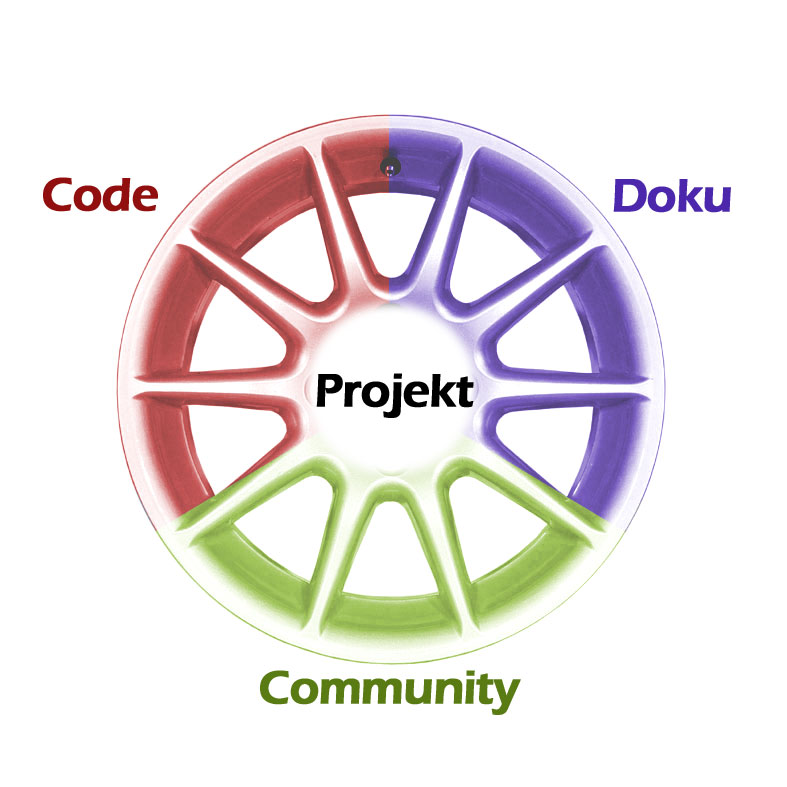
\includegraphics[width=5cm]{cdc}
    \end{column}
    \end{columnsonlytextwidth}
}

\frame{
    \frametitle{Tracing von Open-Source Projekten}
    
    \begin{itemize}
    \item Einheitliche Dokumentation
    \item Architektur sichtbar machen
    \item {\it Wer} hat als letztes {\it was, wo} gemacht?
    \item Qualit�tskontrolle durch Source-Metriken
    \item �berblick �ber die verwendeten Bibliotheken
    \end{itemize}
    
    Das alles, und noch viel mehr: Mit {\bf Apache Maven} in den
    Buildprozess integriert.
}
